\chapter{Zadatak 3b --- četiri slučaja i njihova analiza}
\label{ch:z3-rjesenja}

\section{Što se ovdje traži}

\begin{zadatak}{Zadatak 3, drugi podzadatak}
Riješite problem za 4 različita slučaja: \emph{i)} za slučaj A (parametri zadani
s (2d)) te s $N = 20$; \emph{ii)} za slučaj A s $N = 100$; \emph{iii)} za slučaj B
(parametri zadani s (2e)) te s $N = 20$; \emph{iv)} za slučaj B s $N = 100$.
\end{zadatak}

\begin{predznanje}
\begin{itemize}[nosep,leftmargin=*]
  \item Linearni program \eqref{eq:z3-lp} i matrica $A$ iz \eqref{eq:z3-A}.
  \item Parametri: A ima $b_2 = 0{,}5$, B ima $b_2 = 0{,}2$; $b_1 = 0{,}5$ u oba.
  \item Kako se čita graf --- Poglavlje~\ref{ch:graf}.
\end{itemize}
\end{predznanje}

\section{Kod}
\label{sec:z3-kod}

\begin{seminar}{Seminar v1.2, §4.4 --- ,,(b) Rješenja za četiri zadana slučaja``}
Linearni program rješava se funkcijom \texttt{linprog} uz algoritam dualnog
simpleksa, u petlji po četiri tražena slučaja.

\begin{lstlisting}[style=matlabstyle]
L = 10;
hfun = @(x) 0.0053*x.^4 - 0.095*x.^3 + 0.48*x.^2 - 0.3*x + 1;
opts = optimoptions('linprog', 'Algorithm', 'dual-simplex', 'Display', 'none');

dx = L/N;  x = linspace(0, L, N+1)';  hv = hfun(x);  n = N+1;
f  = [zeros(n,1); dx*ones(n,1)];              % cilj: dx * sum(z)

I  = eye(n);
D1 = (diag(-ones(n,1)) + diag(ones(n-1,1), 1));  D1 = D1(1:N, :)/dx;
D2 = zeros(N-1, n);
for i = 1:N-1
    D2(i, i) = 1;  D2(i, i+1) = -2;  D2(i, i+2) = 1;
end
D2 = D2/dx^2;
Zn = zeros(N, n);  Zc = zeros(N-1, n);

A = [ I, -I;  -I, -I;  D1, Zn;  -D1, Zn;  D2, Zc;  -D2, Zc];
b = [hv;  -hv;  b1*ones(N,1); b1*ones(N,1); b2*ones(N-1,1); b2*ones(N-1,1)];

Aeq = zeros(2, 2*n);  Aeq(1,1) = 1;  Aeq(2,N+1) = 1;
beq = [hv(1); hv(end)];               % rubni uvjeti y0 = a, yN = b
lb  = [-inf(n,1); zeros(n,1)];        % y slobodan, z >= 0

[v, J, ef] = linprog(f, A, b, Aeq, beq, lb, [], opts);
y = v(1:n);
\end{lstlisting}
\end{seminar}

\begin{korak}[Tri retka koja zaslužuju objašnjenje]
\begin{enumerate}[leftmargin=*]
  \item \texttt{lb = [-inf(n,1); zeros(n,1)]} --- donja granica je $-\infty$ za
        $y$ i $0$ za $z$. Bez toga bi niveleta bila prisiljena na nenegativnost.
        Ovdje bi to slučajno bilo neškodljivo (teren je svugdje pozitivan), ali
        bi u općem slučaju tiho promijenilo rješenje.
  \item \texttt{Aeq(1,1) = 1; Aeq(2,N+1) = 1} --- indeksi $1$ i $N{+}1$ su prvi i
        \emph{zadnji} čvor, jer MATLAB indeksira od jedan. Čvor $y_N$ je element
        broj $N+1$.
  \item \texttt{'Algorithm','dual-simplex'} --- simpleks umjesto metode unutarnje
        točke. Za ovaj problem razlika je bitna: simpleks vraća vrh dopustivog
        poliedra, a metoda unutarnje točke točku u sredini optimalnog lica ako
        rješenje nije jedinstveno. O tome više u \S\ref{sec:z3-degeneracija}.
\end{enumerate}
\end{korak}

\section{Rezultati}
\label{sec:z3-rezultati}

\begin{seminar}{Seminar v1.2, Tablica 4.1 --- rezultati za četiri slučaja}
\begin{center}
\begin{tabular}{lcccccc}
\toprule
\textbf{Slučaj} & $N$ & $\Delta x$ [m] & $J^*$ [$\mathrm{m}^2$] & $\max_i |\nabla y_i|$ & $\max_i |\nabla^2 y_i|$ & \textbf{var. / nejed.} \\
\midrule
A ($b_2 = 0.5$) & 20  & 0.50 & $1.916180$ & $0.5000$ & $0.5000$ & 42 / 120 \\
A ($b_2 = 0.5$) & 100 & 0.10 & $1.965940$ & $0.5000$ & $0.5000$ & 202 / 600 \\
B ($b_2 = 0.2$) & 20  & 0.50 & $2.453727$ & $0.5000$ & $0.2000$ & 42 / 120 \\
B ($b_2 = 0.2$) & 100 & 0.10 & $2.506047$ & $0.5000$ & $0.2000$ & 202 / 600 \\
\bottomrule
\end{tabular}
\end{center}

U sva četiri slučaja oba ograničenja dosežu svoju granicu, tj.\ i ograničenje
nagiba i ograničenje brzine promjene nagiba su aktivna.
\end{seminar}

\begin{lstlisting}[style=outputstyle]
Utjecaj mreze  (A): 1.916180 -> 1.965940  (+2.60 %)
Utjecaj mreze  (B): 2.453727 -> 2.506047  (+2.13 %)
Utjecaj b2 (N=100): 1.965940 -> 2.506047  (+27.47 %)
\end{lstlisting}

\begin{korak}[Prva stvar koju treba primijetiti u tablici]
Stupci $\max\abs{\nabla y_i}$ i $\max\abs{\nabla^2 y_i}$ pokazuju \emph{točno}
zadane granice --- $0{,}5$ i $b_2$ --- u sva četiri slučaja. Oba su ograničenja,
dakle, aktivna. To nije slučajnost: teren je na dijelovima trase strmiji od
$b_1$, pa ga niveleta ondje ne može pratiti, a mora doseći zadanu krajnju visinu.
Da nijedno ograničenje nije bilo aktivno, optimalna niveleta bila bi $y = h$ i
trošak bi bio nula.
\end{korak}

\section{Slike i njihovo čitanje}
\label{sec:z3-slike}

\begin{figure}[H]
\centering
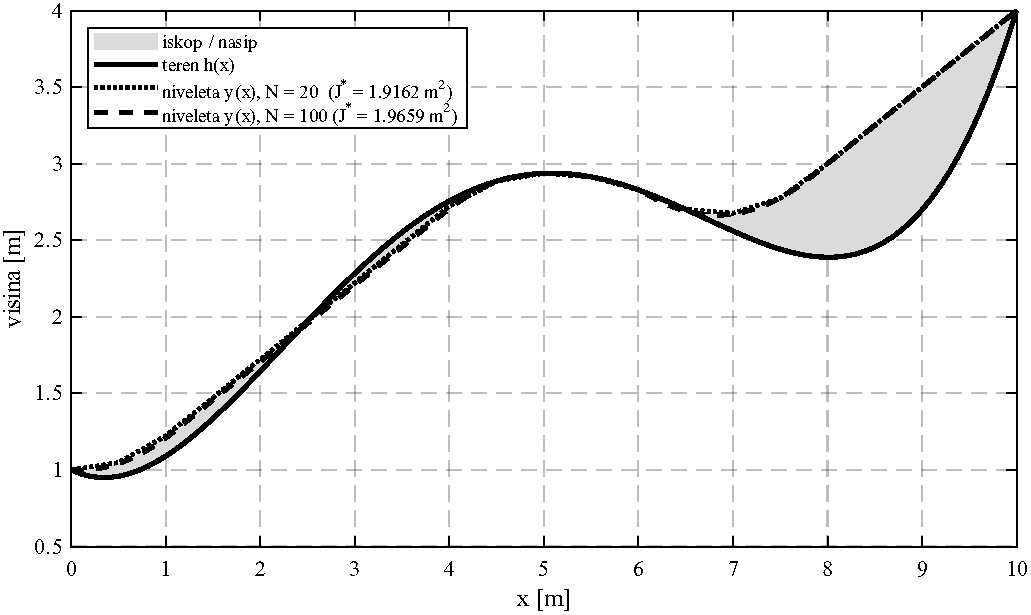
\includegraphics[width=0.92\linewidth]{../figures/fig3_1_road_case_A.pdf}
\caption{Slučaj A ($b_1 = 0{,}5$, $b_2 = 0{,}5\ \mathrm{m}^{-1}$): teren $h(x)$ i
optimalna niveleta $y(x)$ za $N = 20$ i $N = 100$ (Slika 4.1 seminara v1.2).}
\label{fig:z3-A}
\end{figure}

\begin{figure}[H]
\centering
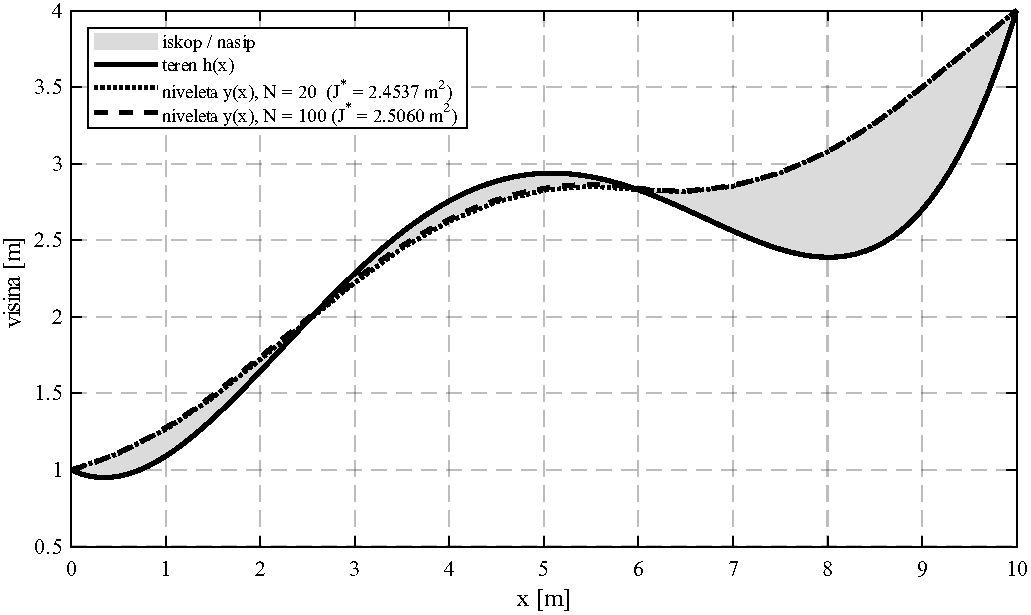
\includegraphics[width=0.92\linewidth]{../figures/fig3_2_road_case_B.pdf}
\caption{Slučaj B ($b_1 = 0{,}5$, $b_2 = 0{,}2\ \mathrm{m}^{-1}$): teren i
optimalna niveleta (Slika 4.2 seminara v1.2).}
\label{fig:z3-B}
\end{figure}

\subsection{Dekonstrukcija}

\begin{longtable}{@{}p{0.30\linewidth} p{0.66\linewidth}@{}}
\toprule
\textbf{Element} & \textbf{Što je i odakle dolazi} \\
\midrule
\endfirsthead
\toprule
\textbf{Element} & \textbf{Što je i odakle dolazi} \\
\midrule
\endhead
Vodoravna os $x$ [m] & Koordinata uzduž trase, $0$ do $L = 10$. \\[5pt]
Okomita os ,,visina`` [m] & Nadmorska visina; raspon otprilike $0{,}5$ do $4$. \\[5pt]
Puna debela krivulja & Teren $h(x)$, zadani polinom četvrtog stupnja. Ima lokalni
maksimum oko $x \approx 5$ i lokalni minimum oko $x \approx 8$. \\[5pt]
Točkasta krivulja & Optimalna niveleta za $N = 20$, s legendom
$J^{\star} = 1{,}9162\ \mathrm{m}^2$. \\[5pt]
Crtkana krivulja & Optimalna niveleta za $N = 100$,
$J^{\star} = 1{,}9659\ \mathrm{m}^2$. Gotovo se poklapa s prethodnom --- razlika
je vidljiva samo lokalno. \\[5pt]
Sivo osjenčano područje & Površina između terena i nivelete, dakle
\emph{iskop ili nasip}. Njezina veličina \emph{jest} vrijednost kriterija. \\[5pt]
Rubovi $x = 0$ i $x = 10$ & Ondje se krivulje dodiruju --- rubni uvjeti traže
$y(0) = h(0)$ i $y(L) = h(L)$, pa odstupanje mora biti nula. \\
\bottomrule
\end{longtable}

\begin{korak}[Zašto niveleta odstupa baš tamo gdje odstupa]
\begin{enumerate}[leftmargin=*]
  \item \textbf{Na kraju trase, $x \in [7, 10]$.} Između $x = 9$ i $x = 10$ teren
        raste za $1{,}30$ m, dakle nagibom većim od $1$. Kako je $y(10) = 4$
        zadano, a nagib nivelete ograničen na $0{,}5$, mora vrijediti
        $y(9) \geq 3{,}5$ i $y(8) \geq 3{,}0$. Ali teren je ondje niži:
        $h(9) = 2{,}698$ i $h(8) = 2{,}389$. Niveleta je stoga prisiljena biti
        \emph{iznad} terena --- odatle najveći nasip na toj dionici, jasno
        vidljiv kao velika siva površina.
  \item \textbf{Na početku, $x \in [0, 3]$.} Teren u okolici $x \approx 2$--$3$
        raste brže od $b_1$, pa niveleta ondje blago odstupa, ali znatno manje.
  \item \textbf{U sredini, $x \approx 4$--$6$.} Ondje se teren i niveleta gotovo
        poklapaju --- teren je sam po sebi dovoljno blag, pa ga se isplati
        pratiti.
\end{enumerate}
\end{korak}

\section{Provjera ograničenja}
\label{sec:z3-provjera}

\begin{figure}[H]
\centering
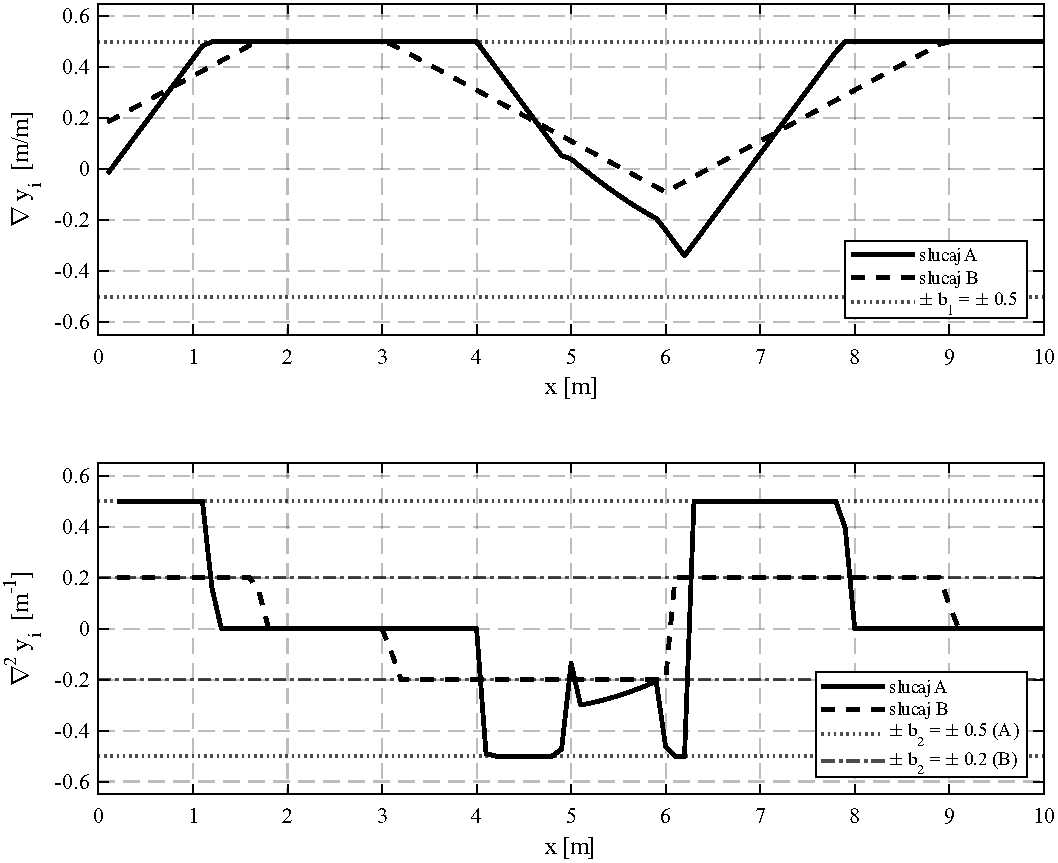
\includegraphics[width=0.90\linewidth]{../figures/fig3_3_road_constraint_check.pdf}
\caption{Provjera ograničenja za $N = 100$: profil nagiba $\nabla y_i$ (gore) i
brzine promjene nagiba $\nabla^2 y_i$ (dolje) za slučajeve A i B (Slika 4.3
seminara v1.2).}
\label{fig:z3-provjera}
\end{figure}

\begin{korak}[Što se s ove slike vidi]
\begin{enumerate}[leftmargin=*]
  \item \textbf{Gornji graf, nagib.} Obje krivulje dodiruju gornju granicu
        $+0{,}5$ na uzlaznim dionicama --- otprilike $x \in [1{,}2,\ 4]$ i
        $x \in [8,\ 10]$. Donju granicu $-0{,}5$ \emph{ne} dodiruju: najniža
        vrijednost je oko $-0{,}34$ (slučaj A) odnosno $-0{,}09$ (slučaj B).
        Dakle ograničenje nagiba je aktivno samo odozgo.
  \item \textbf{Donji graf, druga razlika.} Krivulje su gotovo
        \emph{po dijelovima konstantne}, i to na vrijednostima $+b_2$, $-b_2$ ili
        $0$. To je tipično za rješenje LP-a: optimum je u vrhu poliedra, gdje je
        aktivan maksimalan broj ograničenja, pa varijable ,,sjede`` na granicama.
        Ponašanje se u teoriji upravljanja zove \emph{bang-bang}.
  \item \textbf{Razlika A i B.} U slučaju A druga razlika zasićuje na
        $\pm 0{,}5$ na kratkim odsječcima oko prijelaza. U slučaju B leži na
        $\pm 0{,}2$ duž znatno duljih dionica --- promjena nagiba mora se
        rasporediti na više prostora. To je izravan uzrok većeg volumena
        zemljanih radova.
\end{enumerate}
\end{korak}

\begin{ploca}[Kako skicirati rješenje Zadatka 3 rukom]
\begin{enumerate}[leftmargin=*]
  \item Osi: $x$ od $0$ do $10$, visina od $1$ do $4$.
  \item Nacrtaj teren: kreni iz $(0,\,1)$, blago dolje pa uzbrdo do vrha
        $\approx (5,\ 2{,}93)$, malo dolje do $\approx (8,\ 2{,}39)$, pa strmo
        gore do $(10,\,4)$. To je oblik zadanog polinoma.
  \item Nacrtaj niveletu: poklapa se s terenom na oba kraja i u sredini, a
        odstupa \emph{iznad} terena na dionici $x \in [7, 10]$, jer nagib ne
        smije premašiti $0{,}5$.
  \item Osjenčaj površinu između njih i napiši $J^{\star} \approx 1{,}97\ \mathrm{m}^2$
        (slučaj A) odnosno $2{,}51$ (slučaj B).
  \item Uz dionicu $x \in [8,10]$ napiši računicu: $y(9) \geq 3{,}5$, a
        $h(9) = 2{,}70$ --- to jednom rečenicom objašnjava cijelu sliku.
\end{enumerate}
\end{ploca}

\section{Utjecaj parametara}
\label{sec:z3-analiza}

\subsection{Utjecaj ograničenja $b_2$}

\begin{seminar}{Seminar v1.2, §4.5}
Pooštravanje s $b_2 = 0.5\ \mathrm{m}^{-1}$ (slučaj A) na $b_2 = 0.2\ \mathrm{m}^{-1}$
(slučaj B) prisiljava glađu niveletu: promjena nagiba mora se rasporediti na
dulju dionicu, pa niveleta ranije napušta teren i ne može pratiti njegove
pregibe. Trošak zbog toga raste sa $1.965940$ na $2.506047\ \mathrm{m}^2$ pri
$N = 100$, dakle za $27.47\%$.
\end{seminar}

Ovo je čvrst zaključak: skup dopustivih nivelete za $b_2 = 0{,}2$ je
\emph{podskup} onoga za $b_2 = 0{,}5$ (sve što zadovoljava strožu granicu
zadovoljava i blažu), pa minimum po manjem skupu ne može biti manji. Porast je
zato zajamčen, a njegova veličina --- $27{,}5\%$ --- mjeri koliko udobnost košta.

\subsection{Utjecaj gustoće mreže}

\begin{seminar}{Seminar v1.2, §4.5}
Prelaskom s $N = 20$ na $N = 100$ kriterij raste sa $1.916180$ na
$1.965940\ \mathrm{m}^2$ ($+2.60\%$) u slučaju A, odnosno sa $2.453727$ na
$2.506047\ \mathrm{m}^2$ ($+2.13\%$) u slučaju B. Razlog je u tome što je diskretni
kriterij pravokutna kvadratura po čvorovima: na rijetkoj mreži odstupanje
$|y - h|$ uzorkovano je u malo točaka, pa dio površine između čvorova izmiče sumi
i diskretni kriterij podcjenjuje pravi integral. Pogreška takve kvadrature je
reda $O(\Delta x)$, pa se s pet puta gušćom mrežom vrijednost približava
kontinuiranom integralu.
\end{seminar}

\begin{zamka}[Nijansa: kvadratura nije jedini uzrok, i dvije mreže nisu dokaz reda]
Objašnjenje u seminaru je uvjerljivo, ali nepotpuno, i to je vrijedno znati prije
obrane. Na porast $J^{\star}$ djeluju \emph{dva} učinka istovremeno, a oba guraju
u istom smjeru:
\begin{enumerate}[leftmargin=*]
  \item \textbf{Kvadratura.} Suma po čvorovima podcjenjuje integral, to je točno.
  \item \textbf{Ograničenja postaju stroža.} Diskretna druga razlika preko
        koraka $\Delta x$ je ,,izglađena`` verzija druge derivacije: što je korak
        veći, to je više izglađuje. Na rijetkoj mreži uvjet
        $\abs{\nabla^2 y_i} \leq b_2$ dopušta profile koje bi gusta mreža
        odbacila. Dakle dopustivi skup se s finijom mrežom \emph{steže}, pa i
        zbog toga minimum raste.
\end{enumerate}
Iz dviju mreža ne može se zaključiti ni da je pogreška reda $O(\Delta x)$ --- za
procjenu reda konvergencije treba barem tri mreže i log-log nagib, ili poznato
egzaktno rješenje.

\textbf{Kako odgovoriti ako te se pita:} ,,Porast je posljedica dvaju učinaka
koji djeluju u istom smjeru: pravokutna kvadratura podcjenjuje integral na
rijetkoj mreži, a diskretno ograničenje glatkoće je na rijetkoj mreži blaže nego
na gustoj. Iz dvije mreže mogu tvrditi da vrijednost raste i da je porast malen,
oko dva posto, ali ne mogu odvojiti doprinose ni izmjeriti red konvergencije ---
za to bi trebala serija mreža.``
\end{zamka}

\subsection{Degeneracija: podjela na iskop i nasip}
\label{sec:z3-degeneracija}

\begin{izvor}{Predavanje 5 --- LP i QP, slajd 20/34 (PDF str.~20)}
\slajd[0.86]{p05-simpleks}

\textbf{Transkripcija.} \emph{Simpleks algoritam za rješavanje LP problema.}
Dantzigov simpleks algoritam, autor G.\,B.\ Dantzig, publicirano 1948. godine.
Prema časopisu \emph{Computing in Science and Engineering} jedan od 10
najznačajnijih algoritama 20.\ stoljeća. Ne treba miješati Dantzigovu simpleks
metodu s Nelder--Mead metodom koja se u literaturi isto ponekad zove simpleks
metoda. U današnje vrijeme LP se rješava \emph{metodom unutarnje točke}.
,,Rješavanje LP problema je tehnologija!``

\textbf{Zašto je izbor algoritma ovdje bitan.} Optimalna \emph{vrijednost}
$J^{\star}$ je jedinstvena, ali optimalna \emph{niveleta} ne mora biti. Ondje
gdje se teren i niveleta poklapaju, mali pomak $y_i$ gore ili dolje može ostaviti
zbroj $\sum z_i$ nepromijenjenim --- LP je degeneriran i optimalno lice nije
jedna točka. Simpleks tada vraća neki \emph{vrh} tog lica, a metoda unutarnje
točke točku u njegovoj unutrašnjosti. Zato podjela ukupnog $J^{\star}$ na
,,koliko je iskopa, a koliko nasipa`` nije jedinstvena, i u seminaru su ti stupci
namjerno izostavljeni iz tablice. Ukupni volumen jest jedinstven; njegova
raspodjela nije.
\end{izvor}

\begin{izgovor}
,,Sva četiri slučaja riješena su istim linearnim programom, mijenja se samo
gustoća mreže i granica be dva. U svim slučajevima oba ograničenja su aktivna:
maksimalni nagib je točno nula pet, a maksimalna druga razlika točno be dva.

Rješenje odstupa od terena ondje gdje je teren strmiji od dopuštenog. Najviše na
zadnjoj trećini trase: između devet i deset metara teren raste za metar i trideset,
a niveleta smije najviše nula pet po metru, pa uz zadani rubni uvjet ipsilon od
deset jednako četiri, niveleta mora biti iznad terena --- odatle najveći nasip.

Pooštravanje be dva s nula pet na nula dva povećava trošak za dvadeset sedam i
pol posto. To je zajamčeno, jer je stroži dopustivi skup podskup blažega.

Prelazak s dvadeset na sto podintervala povećava kriterij za oko dva posto.
Tome doprinose dva učinka: pravokutna kvadratura podcjenjuje integral na rijetkoj
mreži, a diskretno ograničenje glatkoće je na rijetkoj mreži blaže. Iz dvije
mreže ne mogu odvojiti ta dva doprinosa.``
\end{izgovor}
